\subsection{RQ2: Which implementation technologies and tools are adopted by software development professionals?}
\label{RQ2}
Our survey included five questions to find technologies and tools that are adopted by software development professionals. To answer this question fully, we report the following results:
\begin{itemize}
\item Technology Platform (Q 9).
\item Operating System (Q 10).
\item Programming Language (Q 11).
\item Framework (Q 12).
\item IDE (Q 13).
\end{itemize}

\subsubsection{Technology Platforms}
Participants were allowed to choose multiple options. As shown in \cref{fig:platforms}, most of the respondents (80\%) worked in web platform. The rests were mobile (45\%), Desktop (30\%), Embedded/IOT (8\%). Most respondents develop products and services for web platforms in both Bangladesh and New Zealand based on \citep{Wang2018}.
\begin{figure}[htbp]
\centering
  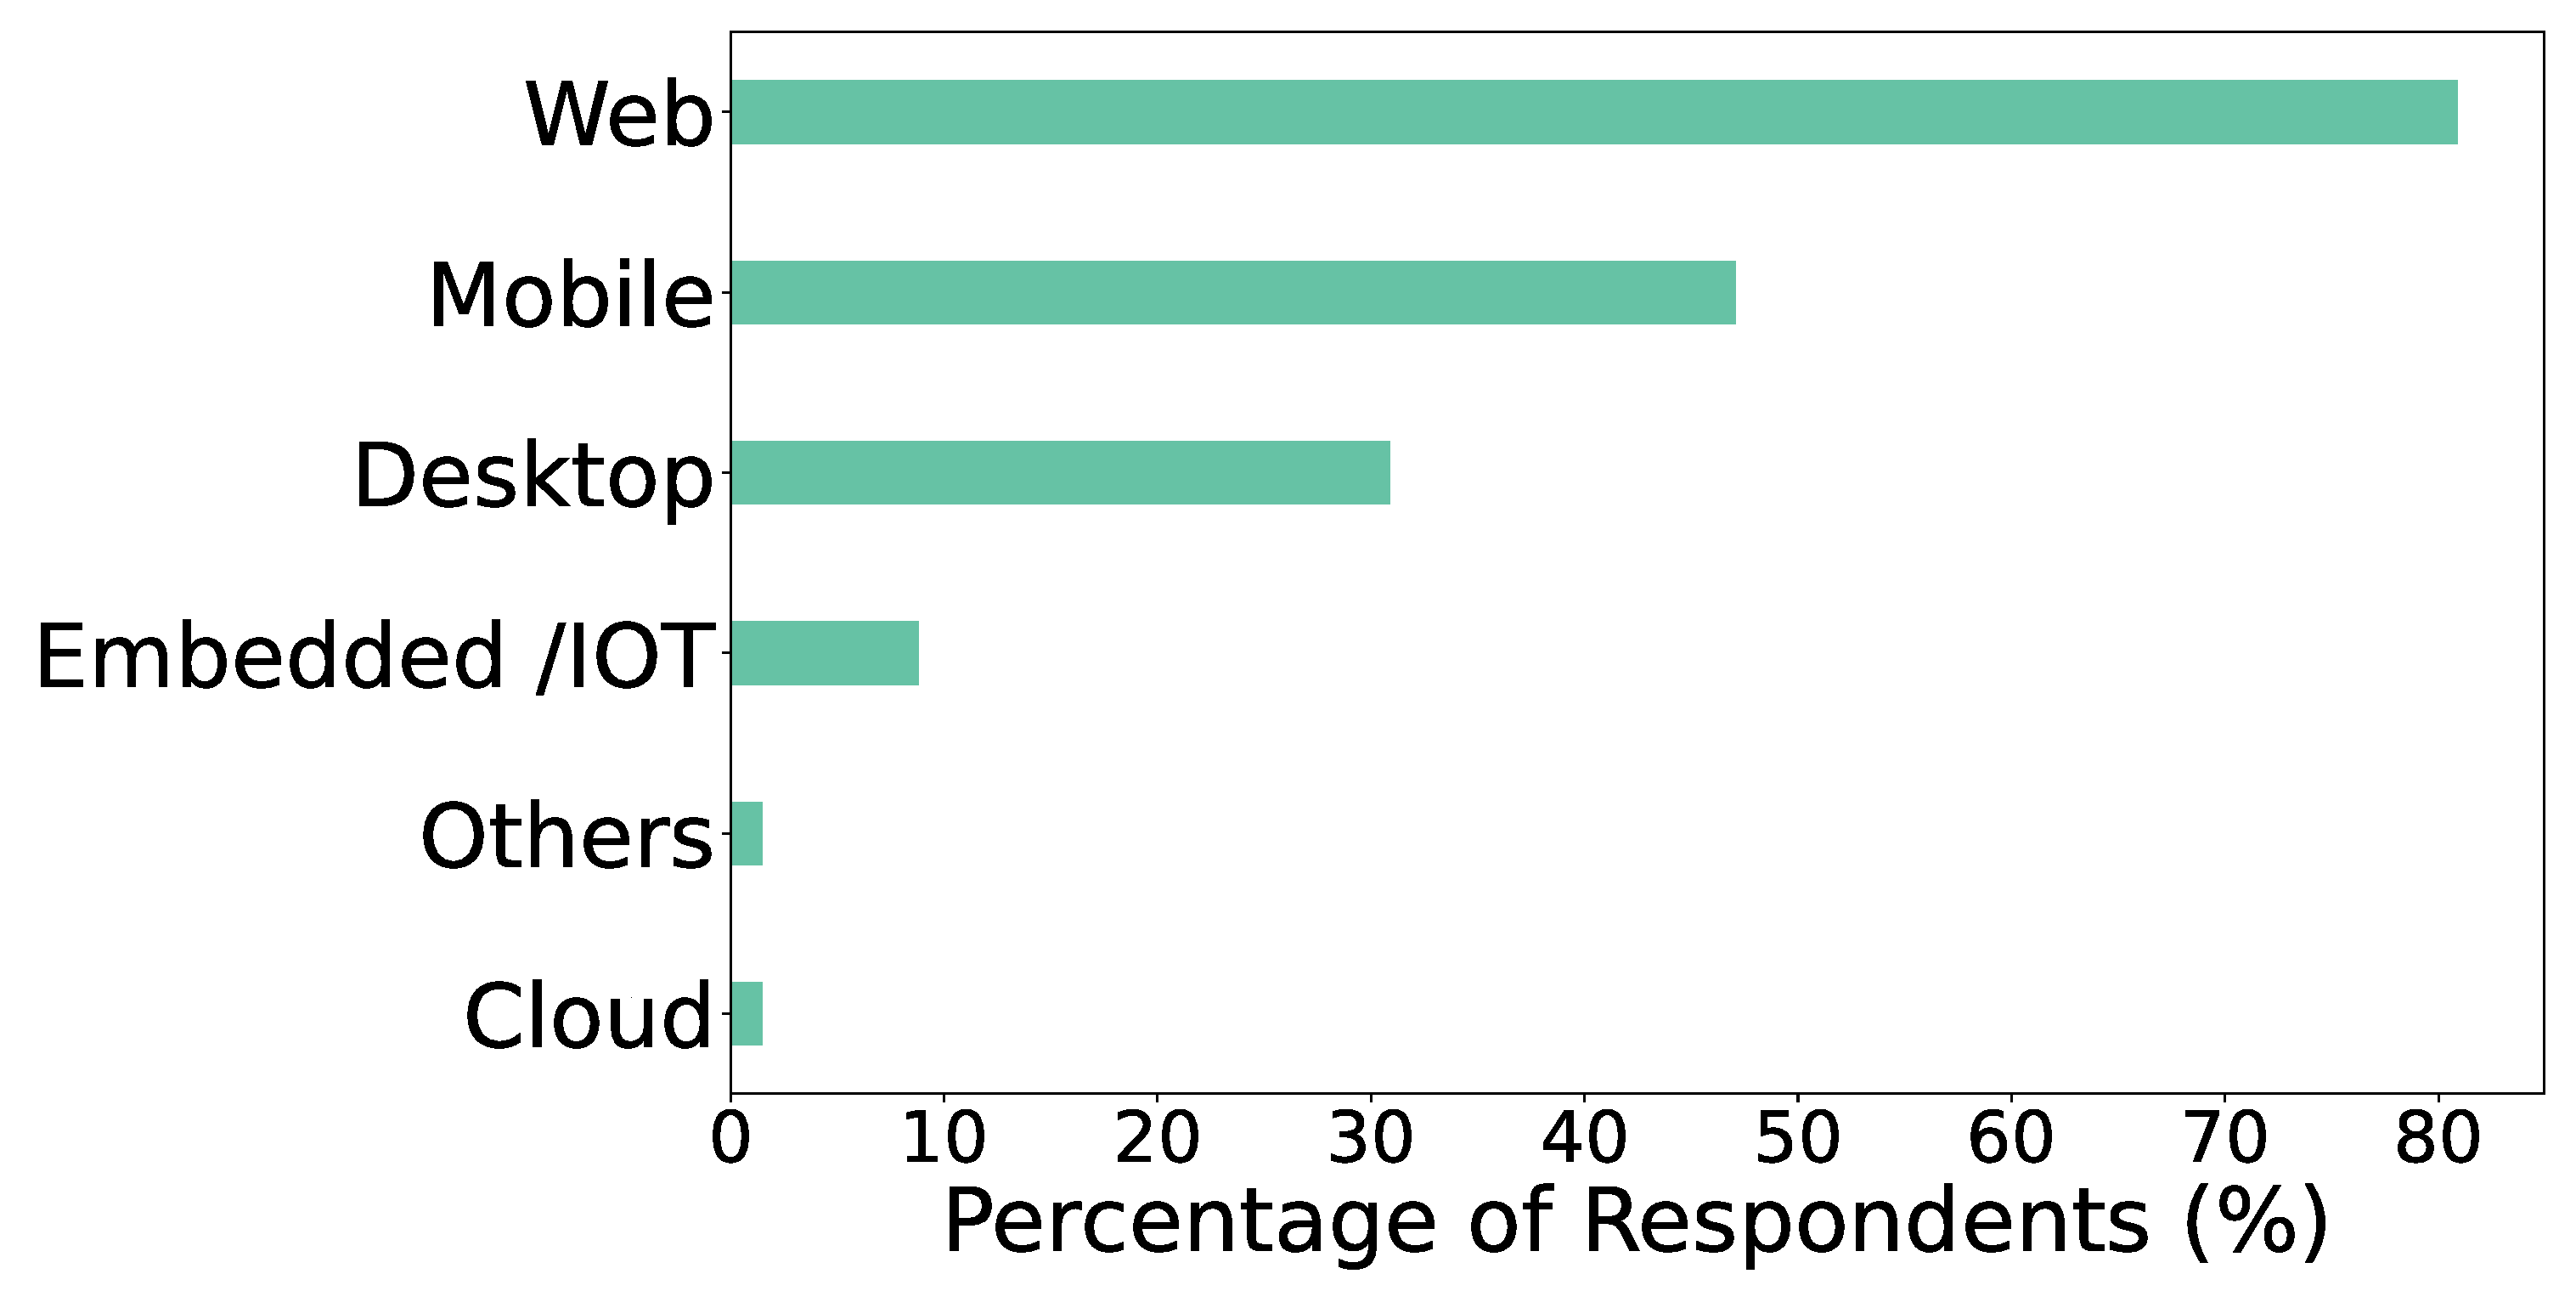
\includegraphics[width=0.8\textwidth]{Figures/Respondents_Technologies}
  \caption{Technology Platforms}
  \label{fig:platforms}
\end{figure}

\subsubsection{Operating Systems}
Most of our respondent's used linux based operating system (56\%). The second best used operating system is windows (45\%). Windows is mostly used among developers of New Zealand based on the survey \citep{Wang2018}, but linux is mostly used in the case for Bangladeshi developers.

\begin{figure}[htbp]
\centering
  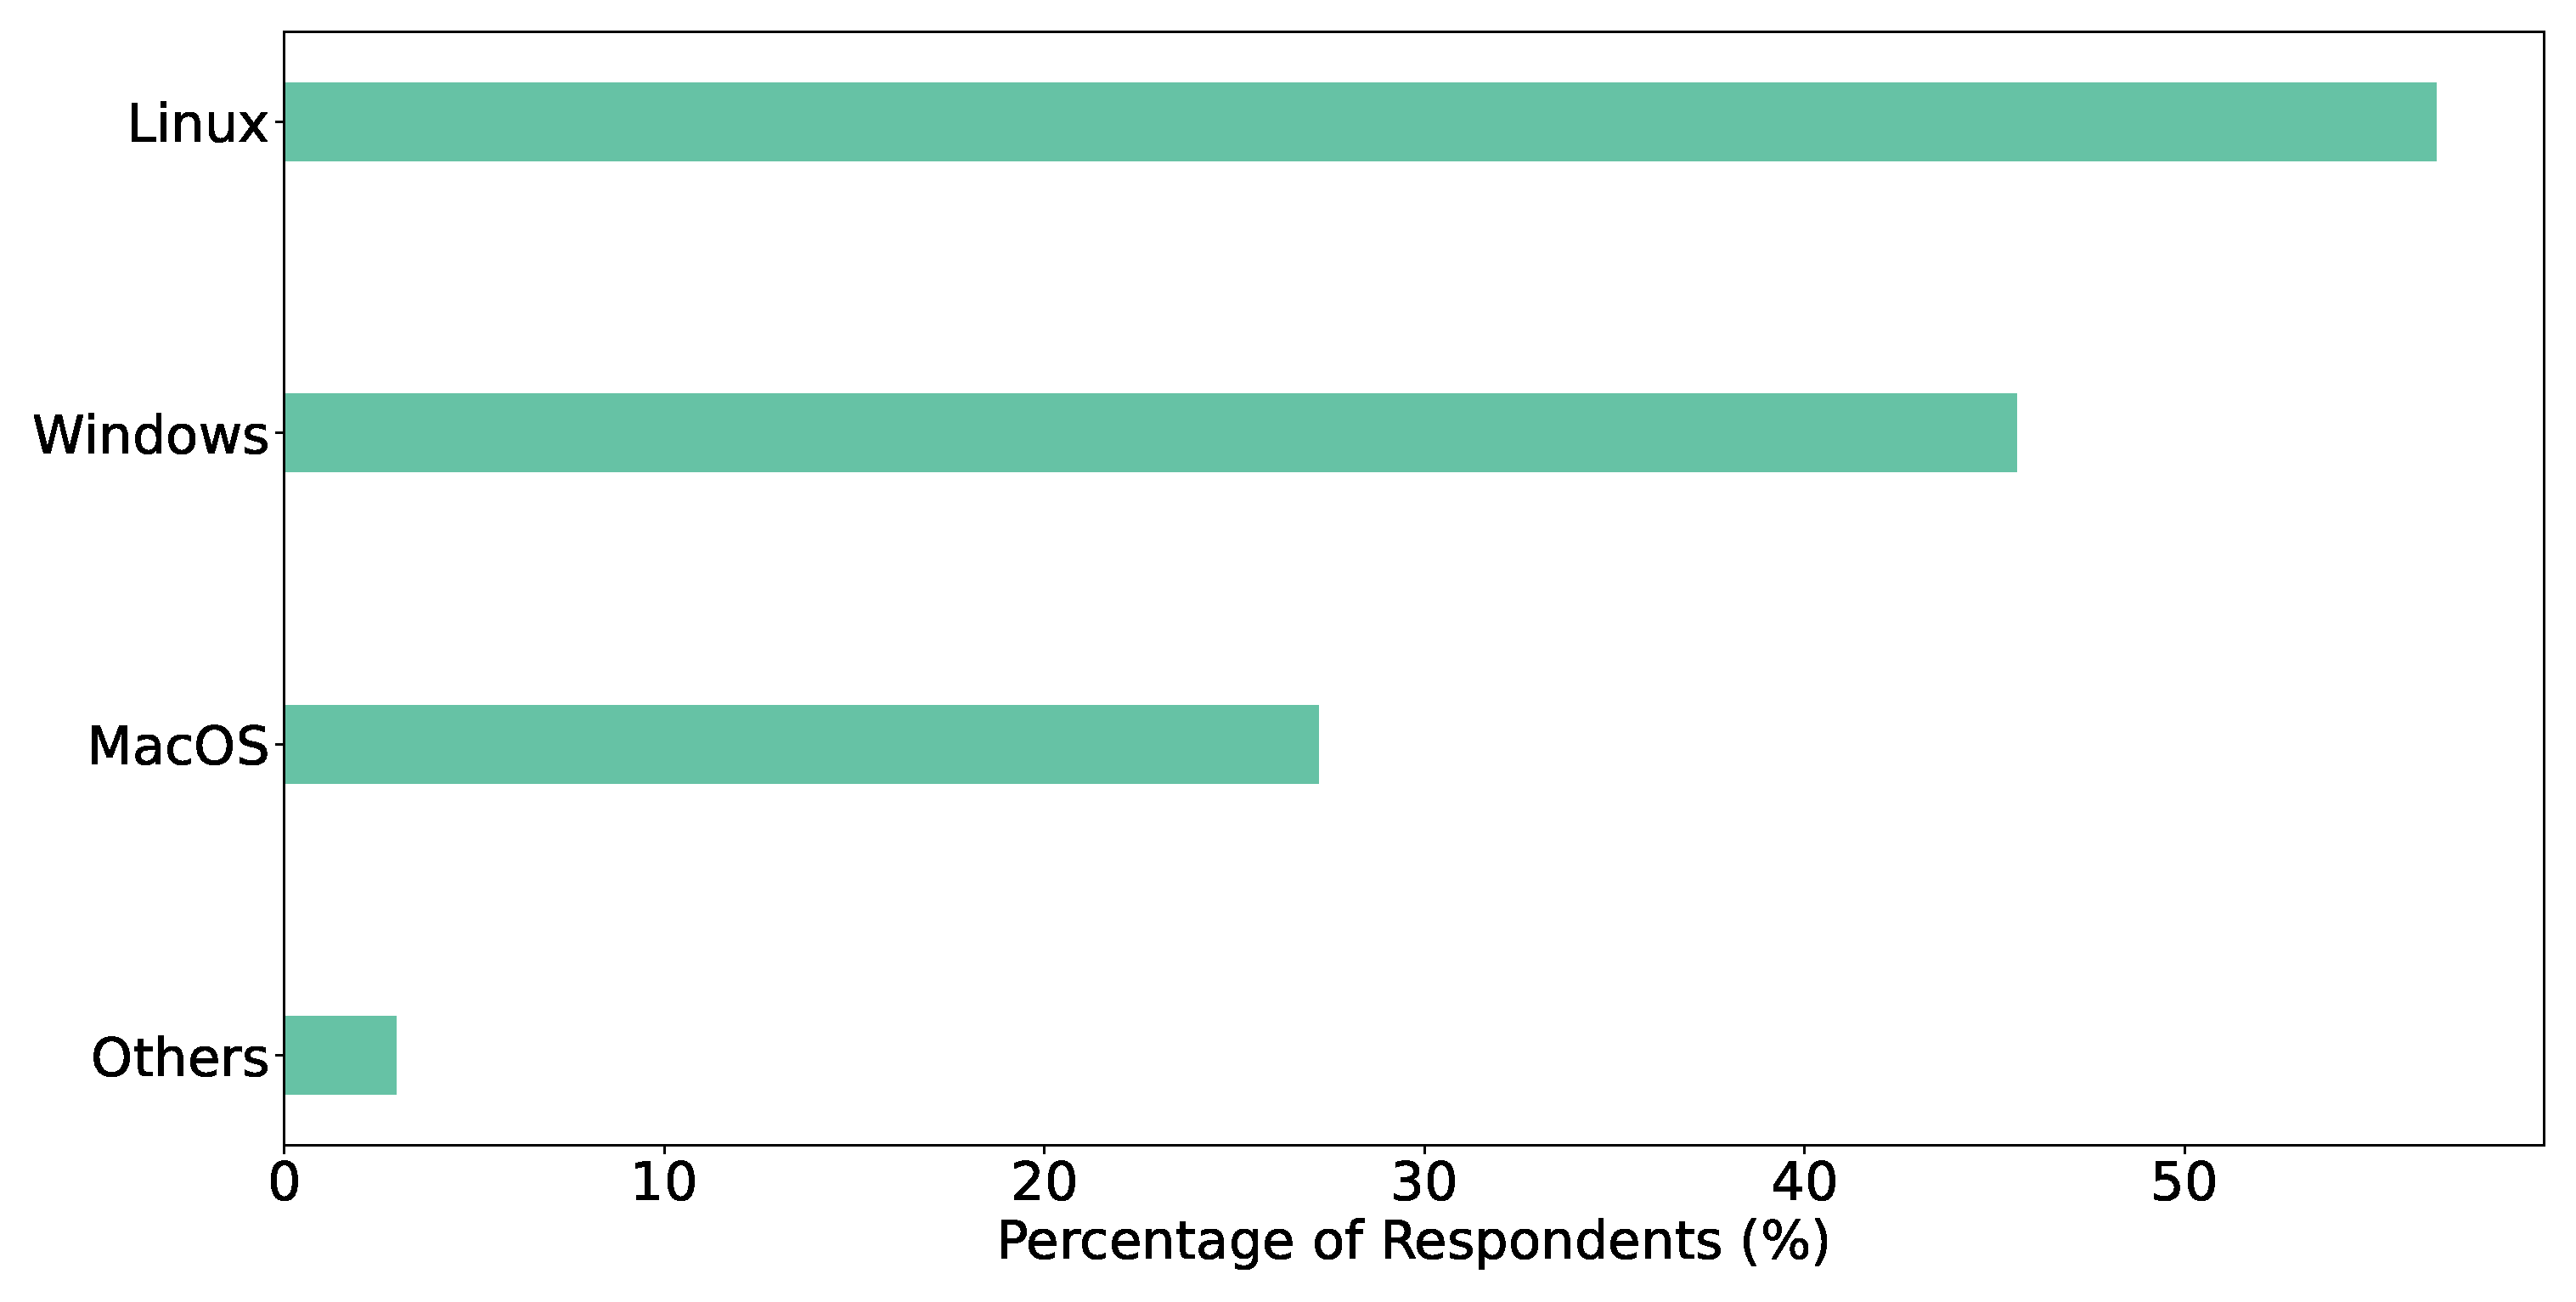
\includegraphics[width=0.8\textwidth]{Figures/Respondents_os}
  \caption{Operating Systems}
  \label{fig:os}
\end{figure}

\subsubsection{Programming Languages}
According to \cref{fig:languages}, around 61\% of our respondent's used Java and Javascript each. Other languages like php (25\%), python (25\%), c\# (18\%) are also used which indicates that the software engineers are not inclined towards a single specific language. Also the choice of programming languages used for development can have important inferences for the testing practices of a software company. Based on \citep{Wang2018}, Java ranks quite low in New Zealand where it is the second most used in Bangladesh and the mostly used language in Turkey \citep{Garousi2015}. Again, python did not get a respective place in the rank of used languages in New Zealand but it is used significantly in Bangladesh.

\begin{figure}[htbp]
\centering
  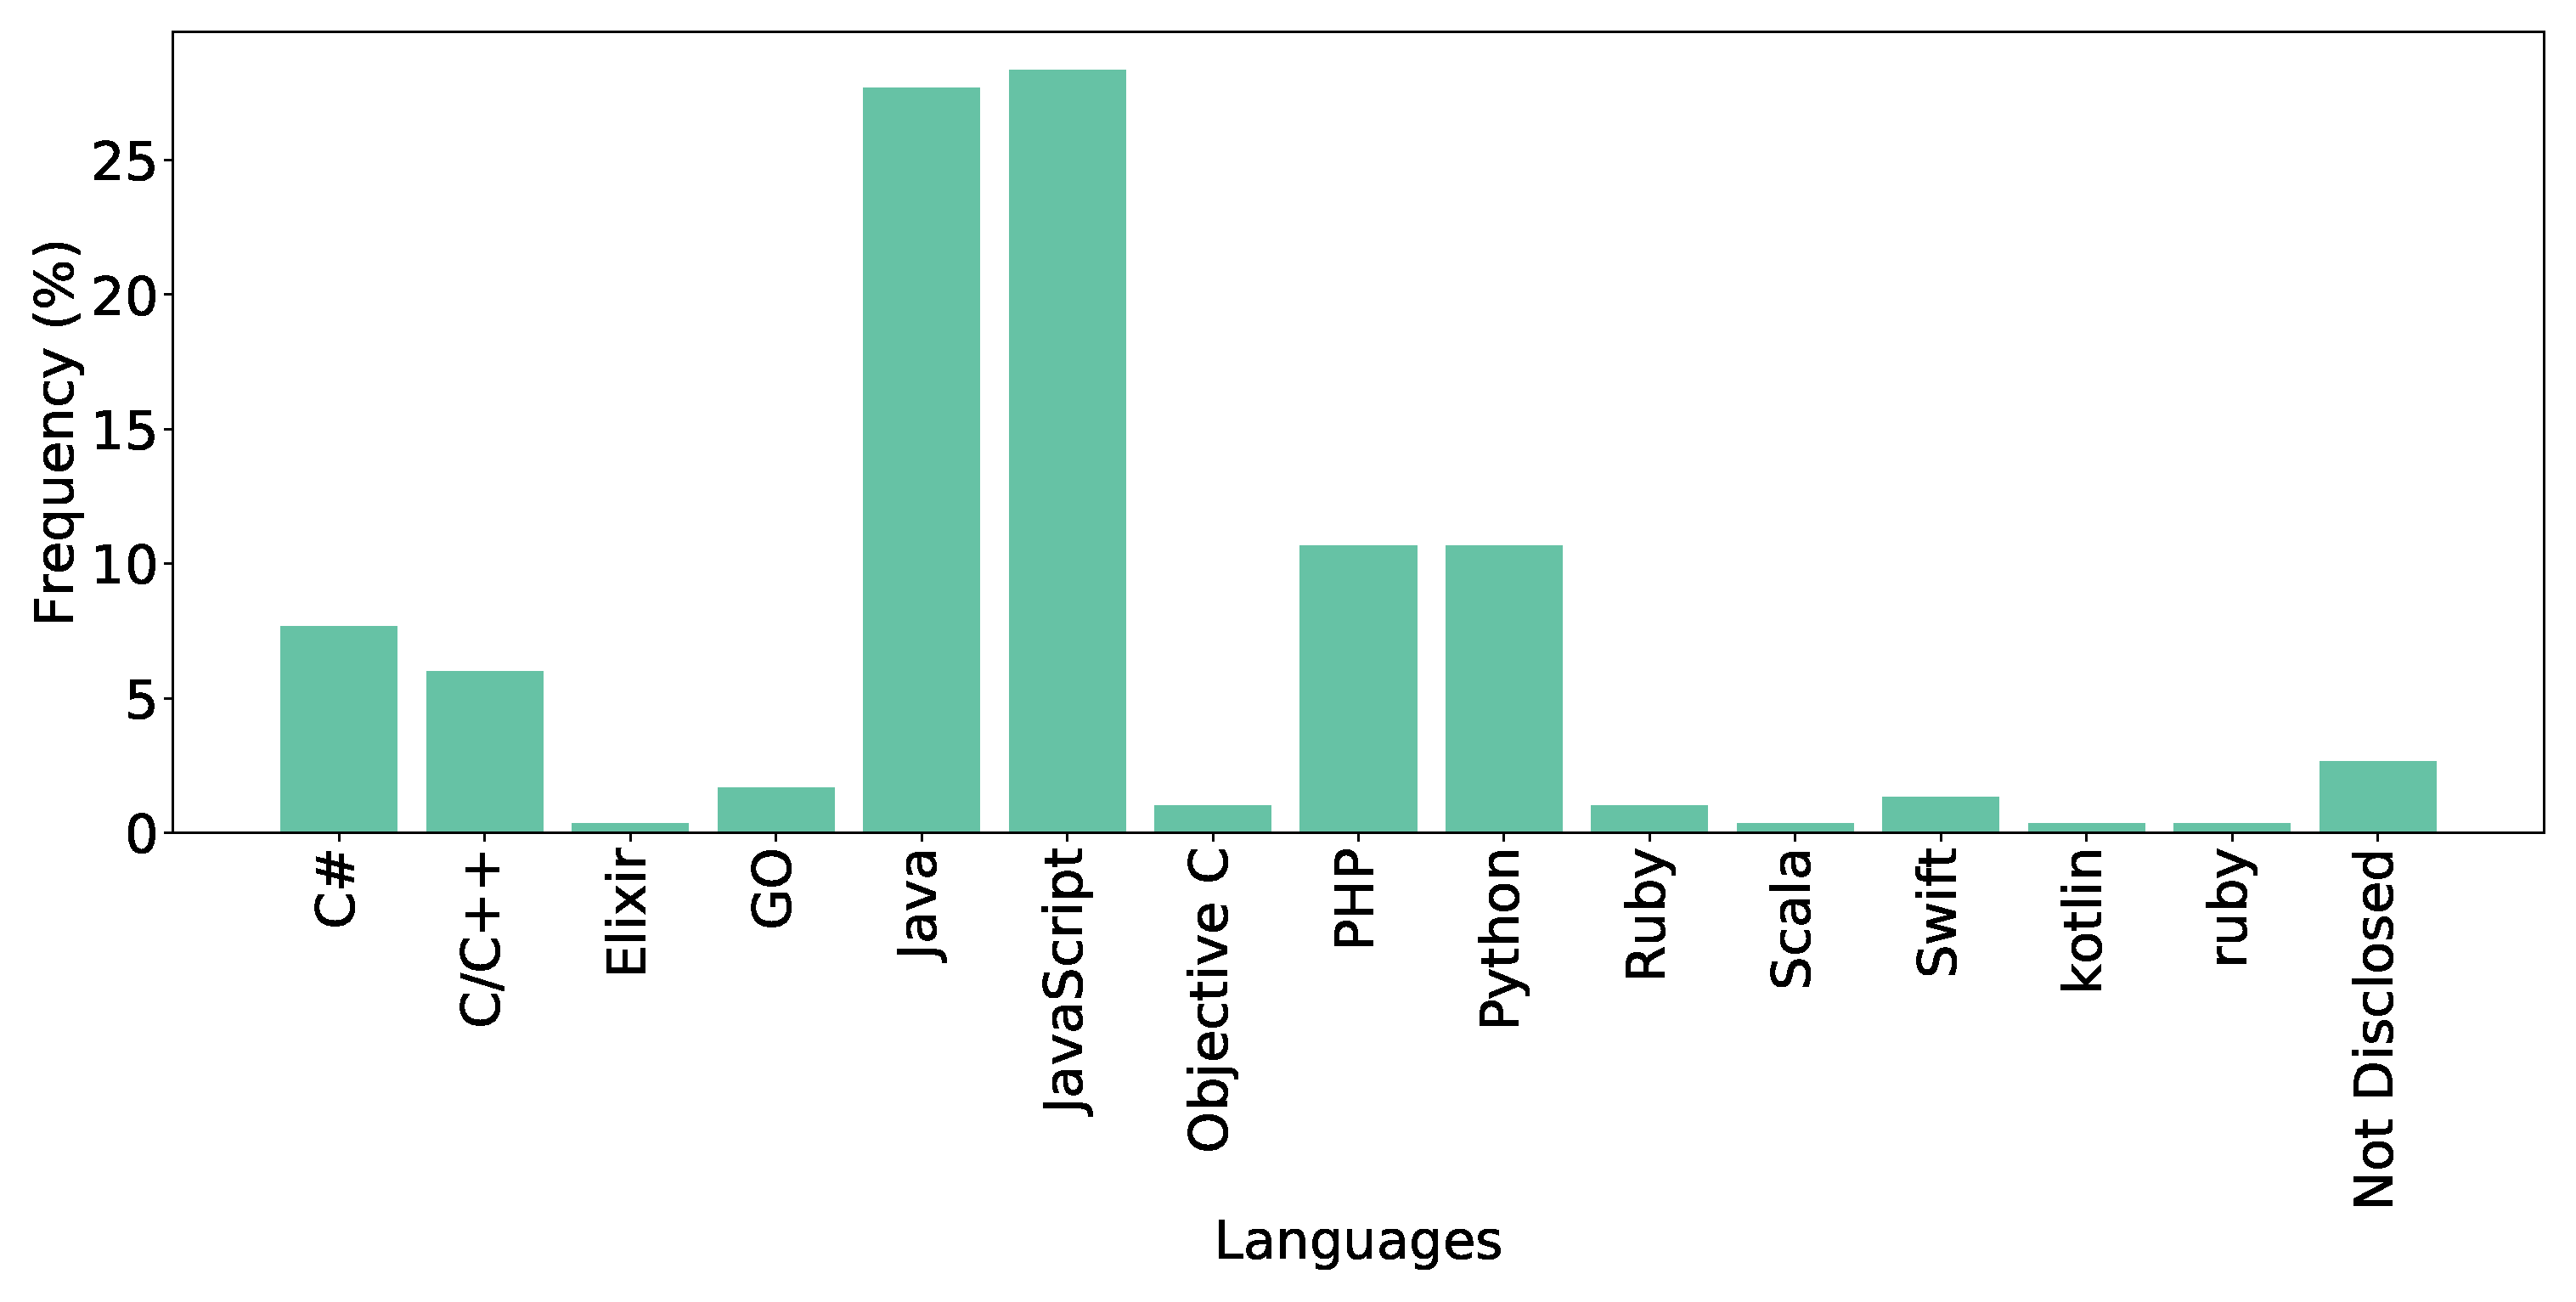
\includegraphics[width=0.8\textwidth]{Figures/Respondents_languages}
  \caption{Languages used in software development}
  \label{fig:languages}
\end{figure}

\subsubsection{Frameworks used in development}
As shown in \cref{fig:frameworks}, variety of frameworks have been used during development. Spring boot (37\%) is the mostly used framework in the industry. ASP.NET, Django and Laravel are used in same proportion (14\%).
\begin{figure}[htbp]
\centering
  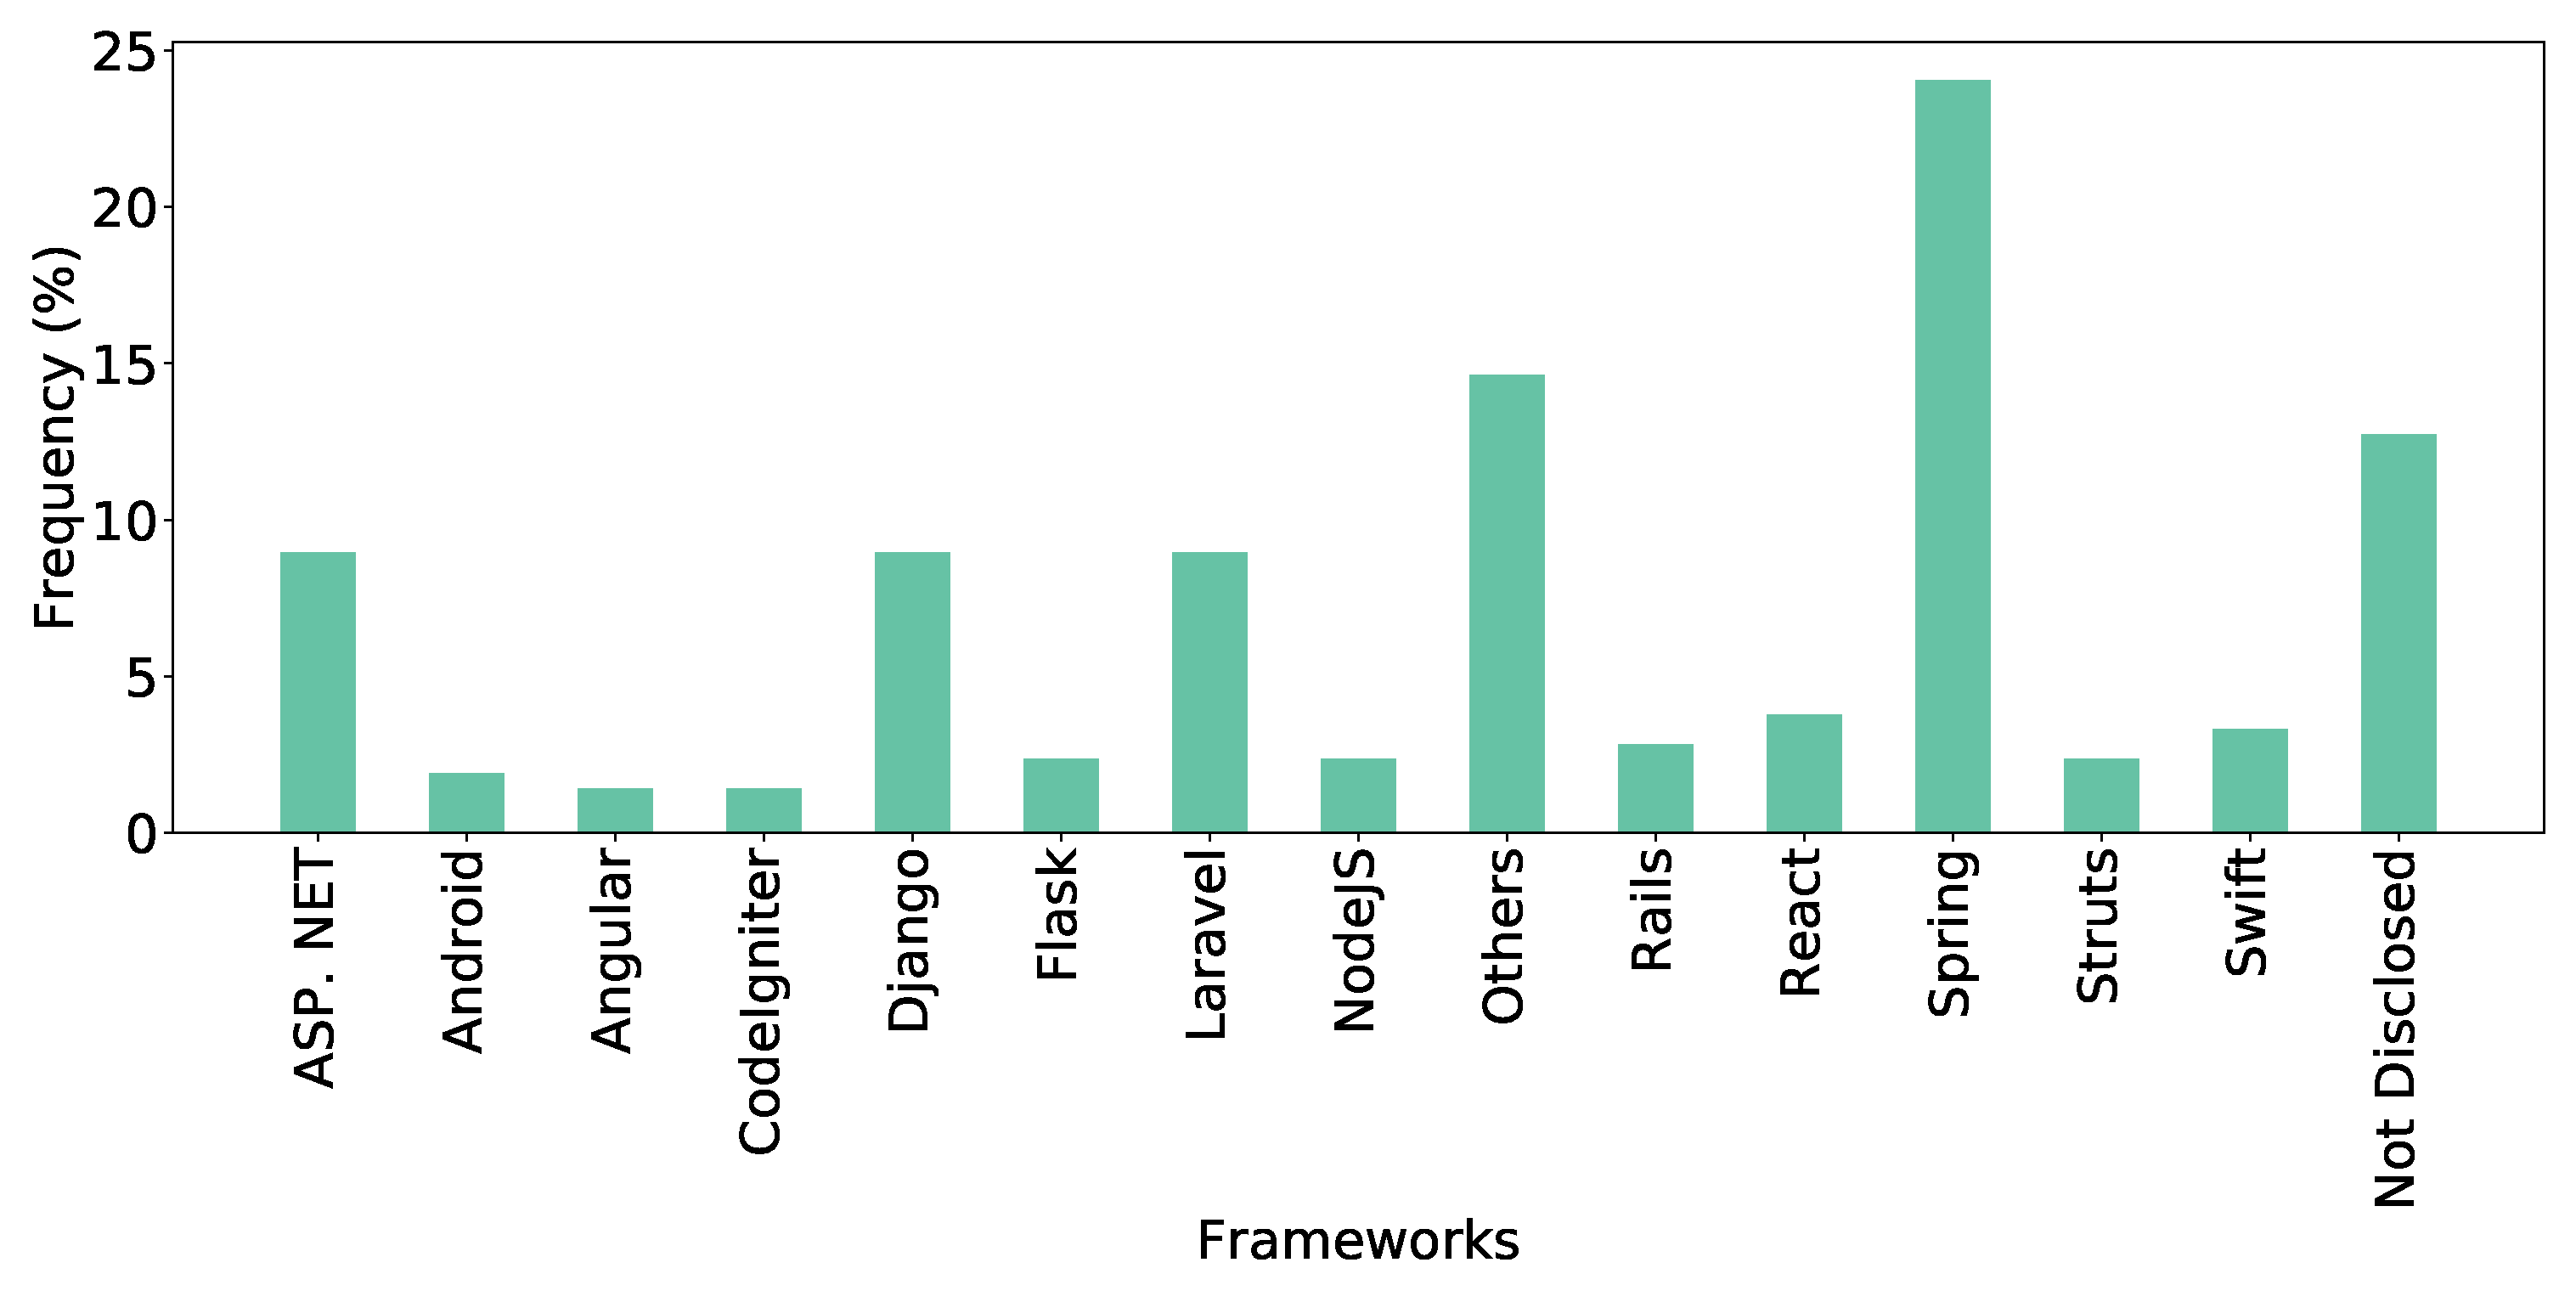
\includegraphics[width=0.8\textwidth]{Figures/Respondents_frameworks}
  \caption{Frameworks}
  \label{fig:frameworks}
\end{figure}

\subsubsection{IDE's used by the respondent's}
According to \cref{fig:IDEs}, IntelliJ, a Java integrated development environment for developing computer software for enterprise, mobile, and web development used by most of the respondents (43\%). The other IDEs used in SE industries are: visual studio (30\%), Eclipse (24\%), PyCharm (16\%), NetBeans (10\%), Android Studio (6\%).
\begin{figure}[htbp]
\centering
  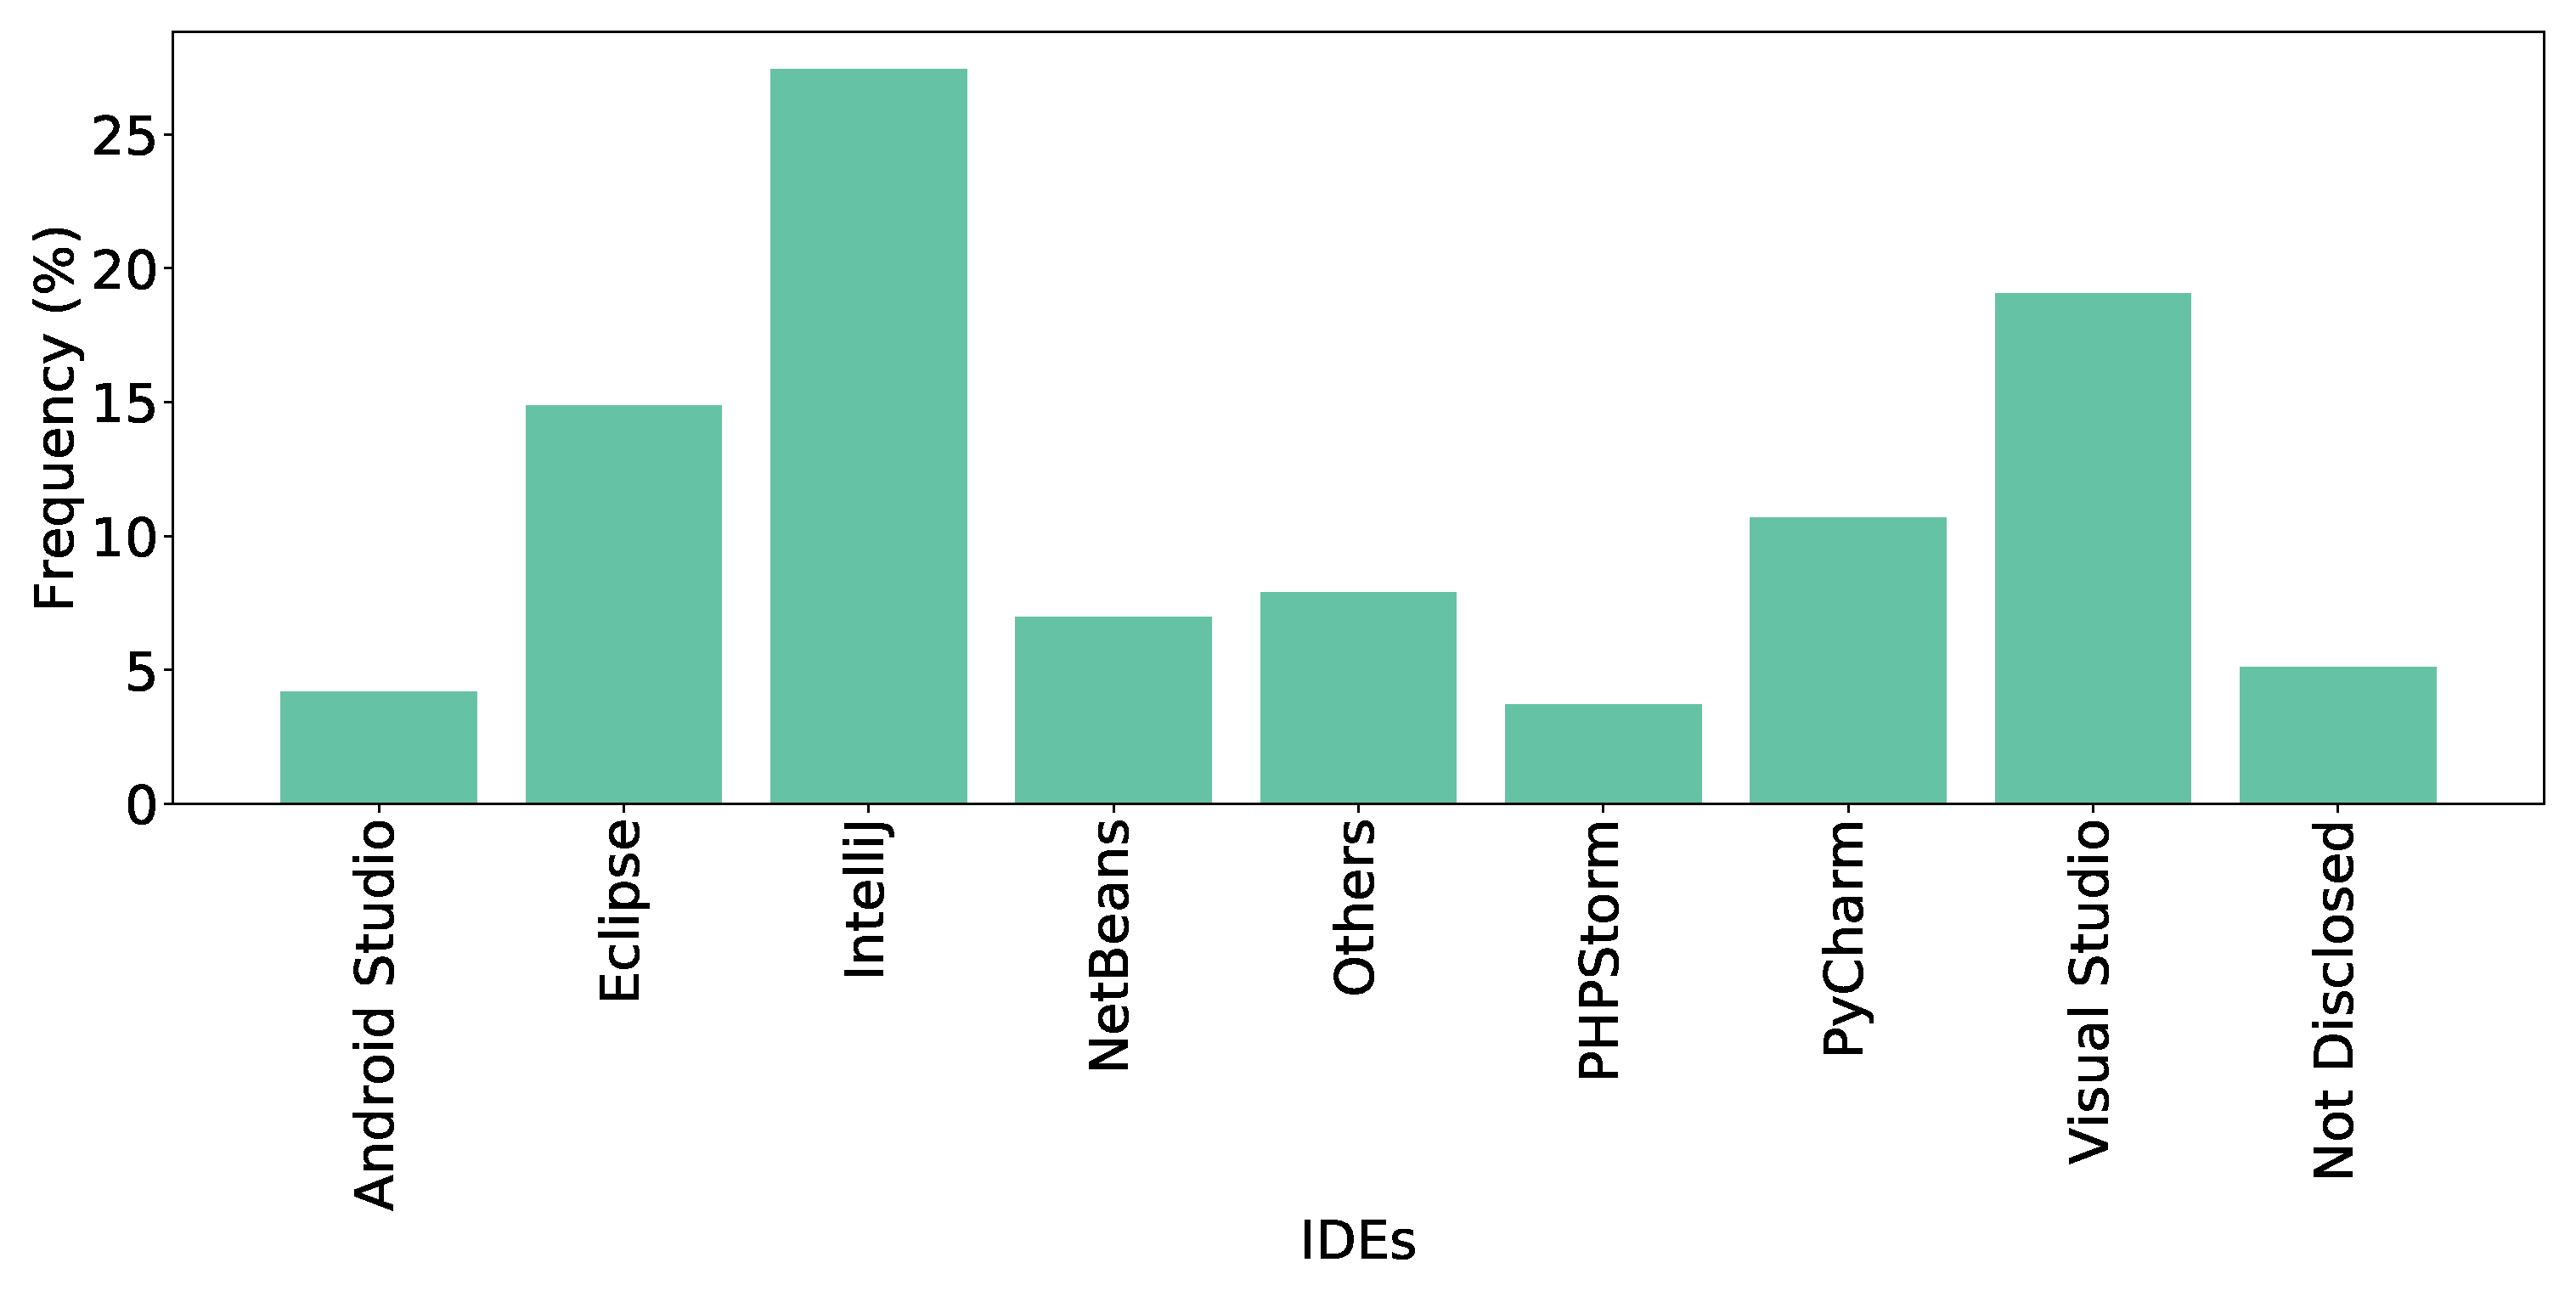
\includegraphics[width=0.8\textwidth]{Figures/Respondents_IDEs}
  \caption{IDE's}
  \label{fig:IDEs}
\end{figure}
